\chapter{Complex Circuits with OpAmps}
\section{Ideal Half-Wave Rectifier}

\begin{figure}
	\centering
	\begin{subfigure}{0.4\textwidth}
		\centering
		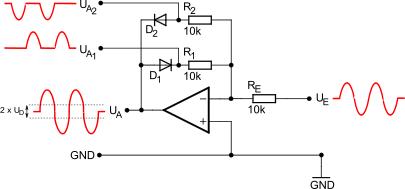
\includegraphics[width=.9\linewidth]{./img/schem-rectifier.pdf}
		\caption{Ideal Rectifier}
		\label{schem:rectfier}
	\end{subfigure}
	\begin{subfigure}{0.4\textwidth}
		\centering
		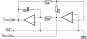
\includegraphics[width=.9\linewidth]{./img/schem-wavegen.pdf}
		\caption{Square and Triangle Wave Generator}
		\label{schem:wavegen}
	\end{subfigure}
	\caption{}
\end{figure}

A basic half-wave rectifier consists of a diode a resistor to provide a load to the diode.
All diodes carry an inherent voltage drop, so the signal level is lowered by \SI{0.2}{\volt} (Schottky diode) to \SI{0.7}{\volt} (silicon diode).

An ideal rectifier (\autoref{schem:rectifier}) uses an operational amplifier with separate feedback paths for the positive and negative half wave.

\section{Square and Triangle Wave Generator}

Operational amplifiers can also be operated with positive feedback.
As any signal is fed back to the input in phase, the output voltage is limited only by the rail voltage of the opamp, and will not remain stable between the rails.

\section{Programmable Differential Equation}
